%!TEX root = ../../main.tex
\section{Experimental methods}
\label{sec:Experimental Methods}

\subsection{Considerations}
\label{sub:Considerations}
To explore the behaviour of $\eta$ as a function of absorbed dose it is necessary to understand the role of $\eta$ in the calculation of the DWD (equation \ref{eq:DWD equation with RDE}).
The crystal is represented as a collection of voxels\footnote{A voxel is the smallest distinguishable volume element in a three-dimensional representation of a computationally modelled object.} in RADDOSE-3D.
$\eta$ is calculated for each voxel within the crystal and the absorbed dose within each voxel is assumed to be homogeneous.
Therefore to experimentally determine the behaviour of $\eta$ within a voxel as a function of absorbed dose, the crystals in the diffraction experiment must be irradiated uniformly to produce a homogeneous dose distribution.
To achieve this it is necessary to use a flat (top-hat) beam profile with the entire crystal volume completely immersed within the X-ray beam throughout the rotation.
At the time of the experiment (January 2014) RADDOSE-3D was only able to model cuboid or spherical crystal shapes.
Therefore the crystals used in the experiment were grown to be as close to cuboid in shape as possible.

\subsection{Crystallization}
\label{sub:Crystallisation}
Crystals of bovine pancreatic insulin purchased from Sigma-Aldrich (Lot \# SLBJ0654V) were grown by the sitting-drop vapour diffusion method.
The well solution consisted of 0.243$\, M$ Na$_{\text{2}}$HPO$_{\text{4}}$, 0.007$\, M$ Na$_{\text{3}}$PO$_{\text{4}}$ at pH 10, and 0.01$\,M$ Na$_{\text{3}}$EDTA.
2$\, \mu l$ of the well solution was added to an equal volume of the protein solution which consisted of 20$\, mg/ml$ insulin protein, 0.0195$\, M$ Na$_{\text{2}}$HPO$_{\text{4}}$, 0.0005$\, M$ Na$_{\text{3}}$PO$_{\text{4}}$ at pH 10, and 0.01$\, M$ Na$_\text{3}$EDTA.
The crystals were stored at room temperature ($\approx$ 293$\,K$) and grew in a morphologically cuboid shape within 48 hours (Figure \ref{fig: Cubic insulin crystals}).
Cuboid shaped crystals less than 140$\, \mu m$ in each dimension were selected and soaked for 30 - 60 seconds in a cryoproctectant solution with an identical composition to that of the well solution except with 30\%$\, v/v$ glycerol substituted for water, before being flash cooled into liquid nitrogen (77$\,$K).
\newline
Human Haspin and myelocytomatosis (MYC) induced nuclear antigen (MINA) protein crystals that were cuboid in shape were kindly provided by the Structural Genomics Consortium (SGC) (Figures \ref{fig: Cubic haspin crytals} and \ref{fig: Cubic MINA crystals}).
These crystals were selected for their cubic shape out of the many human proteins crystallised at the SGC.
They were cryoprotected in their native well solution with 25\%$\, v/v$ glycerol substituted for water.

\begin{figure}
        \centering
        \begin{subfigure}[b]{1\textwidth}
                \centering
                \includegraphics[width=7cm,height=7cm]{figures/dwd/insulin3.png}
                \caption{Insulin}
                \label{fig: Cubic insulin crystals}
        \end{subfigure}
				\\
        \begin{subfigure}[b]{1\textwidth}
                \centering
                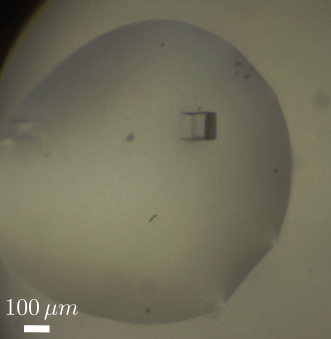
\includegraphics[width=7cm,height=7cm]{figures/dwd/haspin2.png}
                \caption{Haspin}
                \label{fig: Cubic haspin crytals}
        \end{subfigure}
				\\
        \begin{subfigure}[b]{1\textwidth}
                \centering
                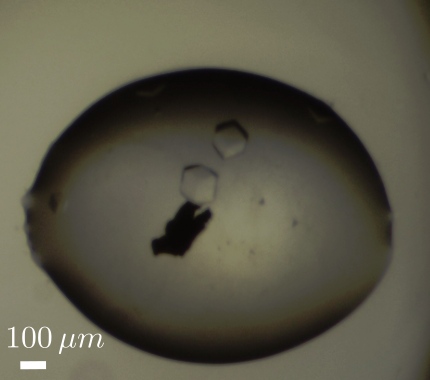
\includegraphics[width=7cm,height=7cm]{figures/dwd/mina2.png}
                \caption{MINA}
                \label{fig: Cubic MINA crystals}
        \end{subfigure}
				\caption[Crystals used in the experiment at PETRA III, Hamburg]{Crystals used in the experiment.}
        \label{figcrystals}
\end{figure}

\subsection{Data collection and dose calculation}
\label{sub:Data Collection and Dose Calculation}
All data were collected at 100\,K on the PETRA III Hamburg beamline P14 using an X-ray energy of 12.7\,keV ($\lambda = \text{0.9764}\,$\AA), in collaboration with beamline scientist Dr. Gleb Bourenkov and EMBL beamline director Dr. Thomas Schneider.
The experimentally measured beam profile was determined by placing a scintillator combined with an Allied Vision GC1350C CCD camera directly in the beam path.
This produced a quantitative map of the beam profile in a portable graymap (pgm) file.
The flat profile of the beam (coefficient of variation\footnote{The coefficient of variation is defined at the ratio of the standard deviation to the mean of a set of values which can also be expressed as a percentage by multiplying by 100\%.} of the beam is 2.09\% vertically and  2.24\% horizontally) was achieved by removing the focusing mirrors, and the slits were adjusted to achieve an aperture of 140$\,\mu m \times $140$\,\mu m$ (Figure \ref{fig: Hamburg beam pgm and slice}).
The beam current was measured using a 500$\,\mu m$ thick silicon PIN diode placed in the sample position from which the photon flux could be calculated \cite{owen2009}.
Before the data were collected from each crystal, an indexing set (100 frames of 0.1$^{\circ}$ rotation and 0.1$\,s$ exposure time per frame) was acquired.
These frames were then indexed to provide the information necessary to reorient the crystal.
One of the crystal faces was then aligned perpendicular to the beam direction such that the plane containing the beam direction vector was perpendicular to two of the edges of the aligned face (Figure \ref{fig: indexing flow diagram}).
Alignment was performed using an Arinax MD3 mini kappa goniometer with the spindle axis mounted in a vertical and downward configuration.
The crystal was centred on the beam position to make sure the entire crystal volume was completely immersed in the beam during the experiment.
The dimensions of the crystals were measured on the screen prior to data collection.
Table~\ref{tab:Hamburg data collection} contains the details of the data collection strategies for each crystal type.

Dose values were calculated using RADDOSE-3D.
The photon flux was determined to be 1.9 $\times$ 10$^{\text{11}}\,ph/s$, the composition of the crystal was obtained from Dr. Oliver B. Zeldin's thesis \cite{zeldin2013thesis} and from the constituents of the crystallisation solution as in Section \ref{sub:Crystallisation}.
Although the crystal composition in Zeldin's thesis is incorrect (he specifies that there is a zinc atom for every insulin monomer in the unit cell whereas the true composition has only two zinc atoms per insulin hexamer), using the same composition allows direct comparison with the results obtained in \cite{zeldin2013dwd}.
Functionality to handle the experimentally measured beam profile was added to RADDOSE-3D to further improve the simulation of the absorbed dose.
\begin{figure}
        \centering
        \begin{subfigure}[b]{1\textwidth}
                \centering
                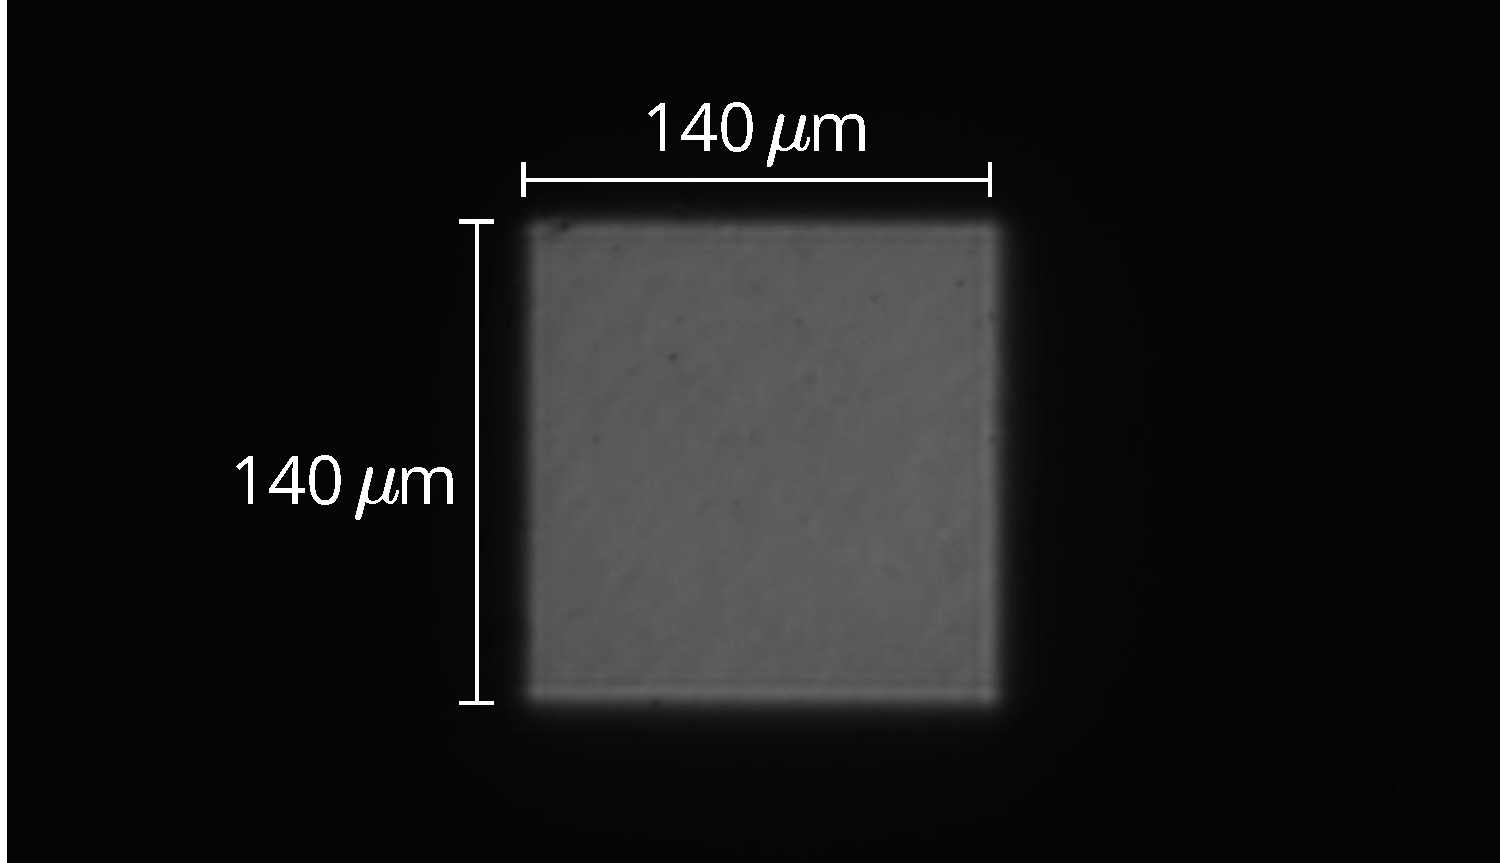
\includegraphics[width=\textwidth]{figures/dwd/hamburg_beampgm.pdf}
                \caption{}
                \label{fig: Hamburg beam PGM}
        \end{subfigure}
				\\
        \begin{subfigure}[b]{1\textwidth}
                \centering
                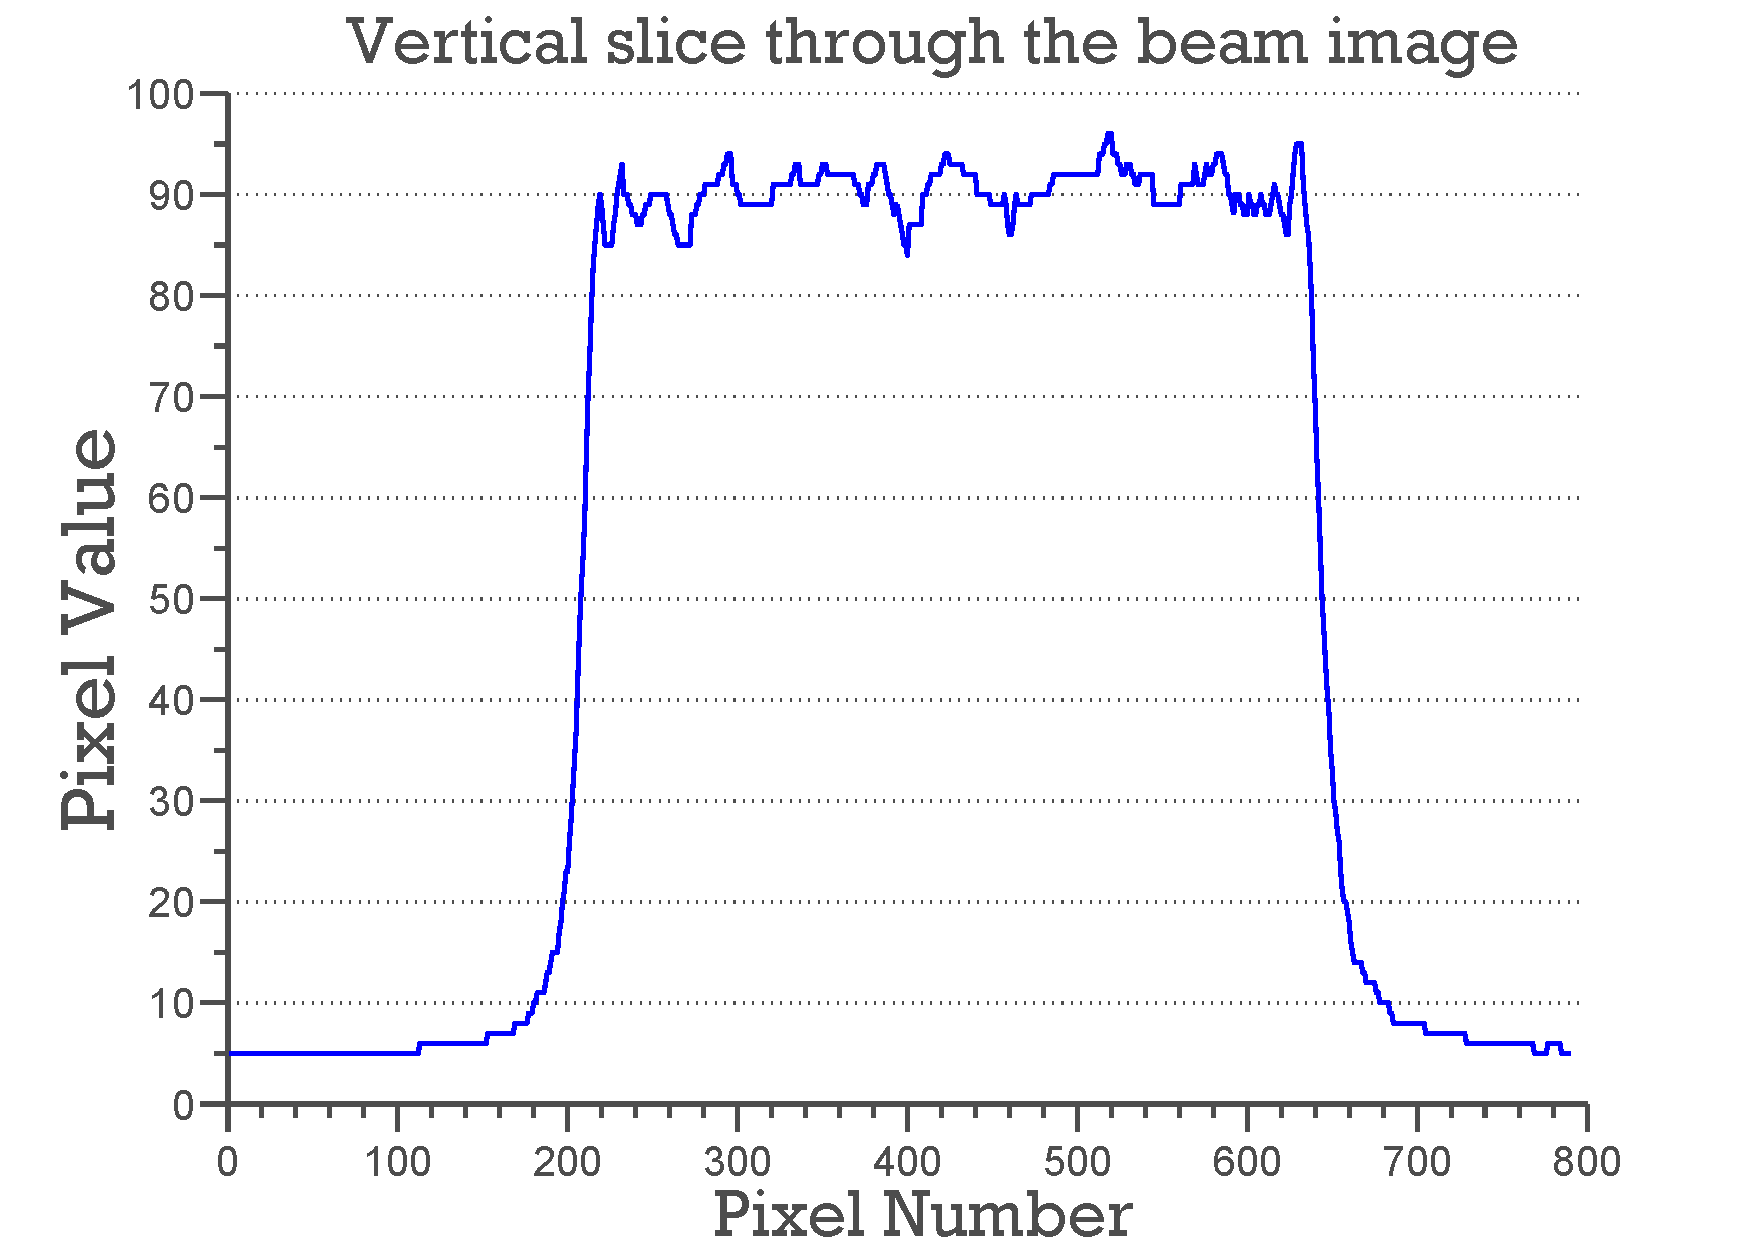
\includegraphics[width=\textwidth]{figures/dwd/beamslice.pdf}
                \caption{}
                \label{fig:Hamburg beamslice}
        \end{subfigure}
\end{figure}
\begin{figure}
    \ContinuedFloat
    \begin{subfigure}[b]{1.0\textwidth}
        \centering
        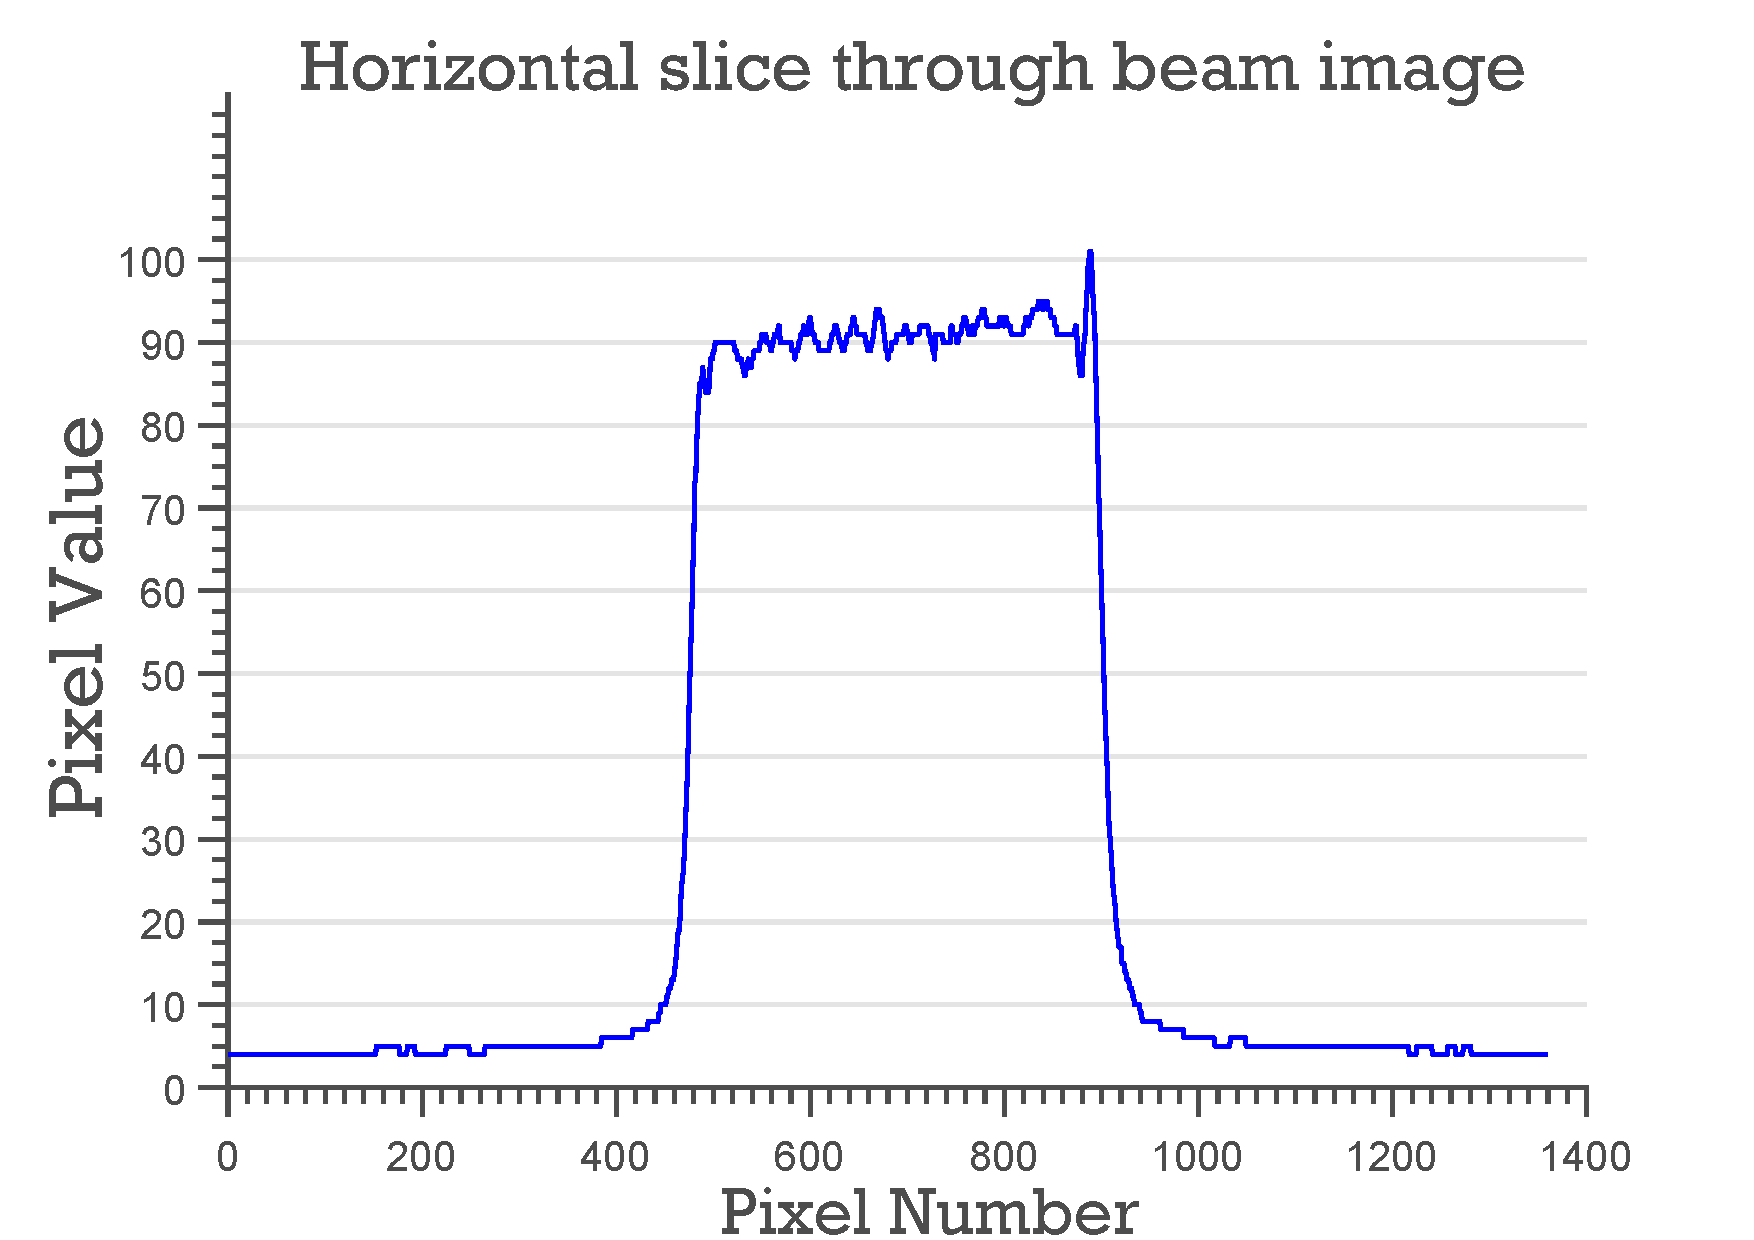
\includegraphics[width=\textwidth]{figures/dwd/beamslice_horizontal.pdf}
        \caption{}
        \label{fig:Hamburg beamslice horizontal}
    \end{subfigure}
    \caption[Beam profile at beamline P14, PETRA III, Hamburg.]{(a) Image (790 x 1360) of the experimentally determined beam profile.
    (b) Vertical slice through the beam image showing the flat profile of the beam.
    (c) Horizontal slice through the beam image showing the flat profile of the beam.}
    \label{fig: Hamburg beam pgm and slice}
\end{figure}

\begin{figure}
  \centering
    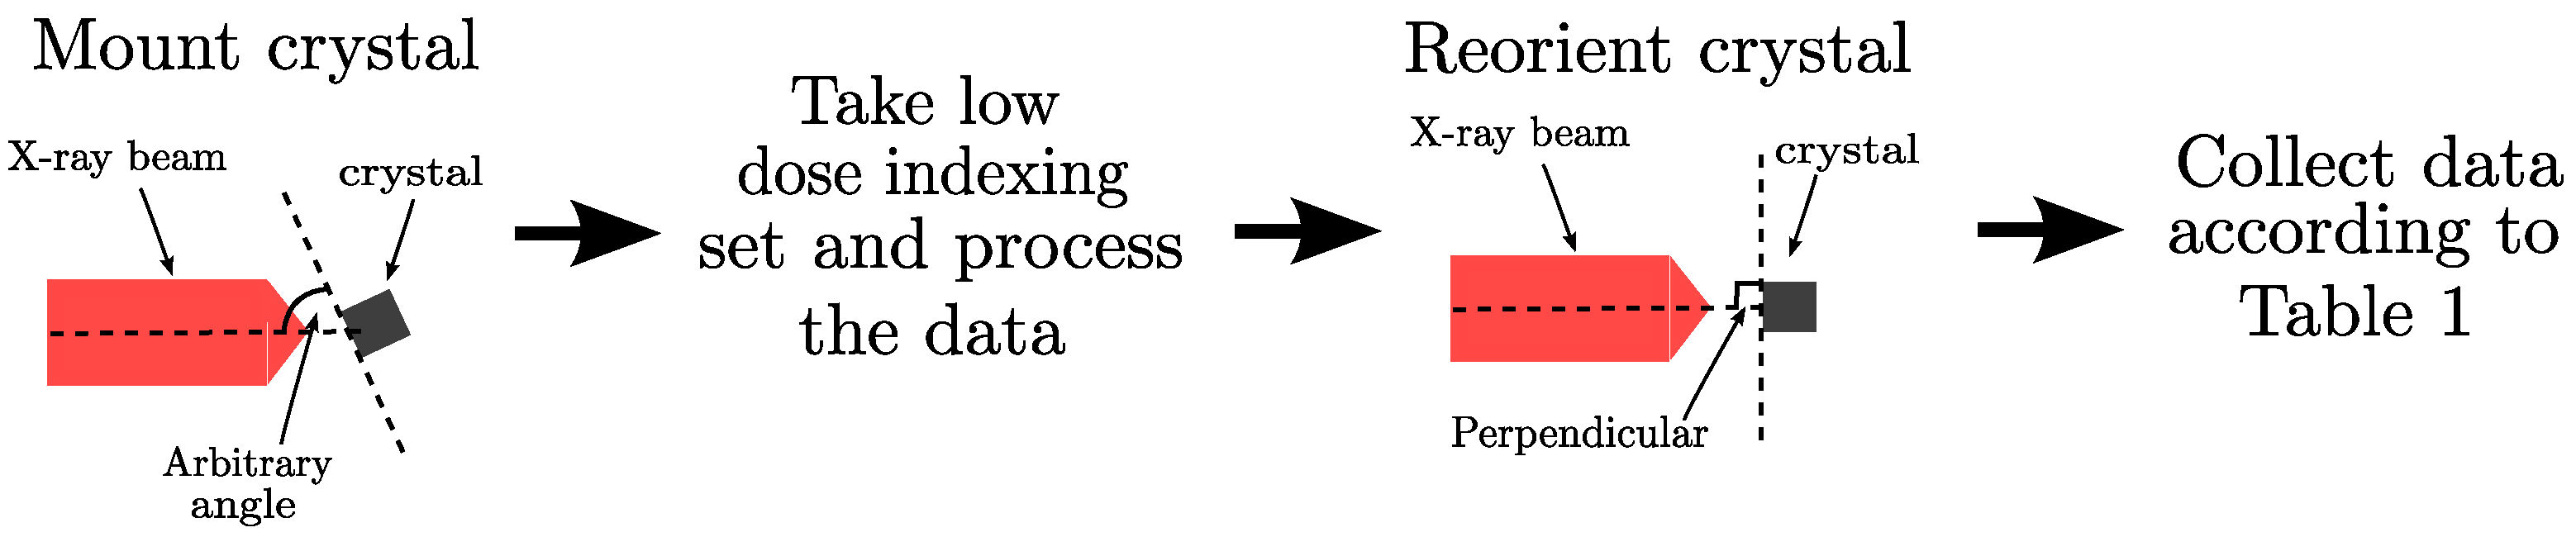
\includegraphics[width=1\textwidth]{figures/dwd/initial_indexing.pdf}
    \caption[Flow diagram of the crystal reorientation process prior to data collection at PETRA III.]{Flow diagram of the crystal reorientation process prior to data collection.}
    \label{fig: indexing flow diagram}
\end{figure}

\begin{table}[ht!]
	\caption[Data collection strategy for each protein crystal type at PETRA III.]{Data collection strategy for each protein crystal type}
	\centering
	\begin{tabular}{p{1.6cm} p{1.4cm} p{2.0cm} p{1.3cm} p{1.5cm} p{2.0cm} p{2.0cm}}
		\hline
		Protein Crystal Type & Number of Crystals & Total Number of Frames per crystal & Rotation per image ($^\circ$) & Total rotation ($^\circ$) & Exposure Time per image (seconds) & Approx resolution \\
		\hline
		Insulin      & 8   & 14400  		& 0.1 & 1440    & 0.5 & 1.38$\,$\AA \\
		Haspin       & 5   & 7200   		& 1   & 7200    & 1   & 2.9$\,$\AA\\
		MINA         & 3   & 7200/3600      & 0.1 & 720/360 & 1   & 3.0$\,$\AA\\
		\hline
	\end{tabular}
	\label{tab:Hamburg data collection}
\end{table}

\subsection{Data processing}
\label{sub:Data Processing}
The data collected for the SGC MINA and haspin crystals were non-trivial to analyse and hence the data processing procedures described here are relevant only for the insulin crystals.
Data were processed using the Collaborative Computational Project No. 4 (CCP4) suite \cite{winn2011} with a standardised script used to call each program from within the suite to ensure identical treatment of all crystals.
MOSFLM \cite{leslie2007} was run manually with the space group set to $I$2$_{\text{1}}$3.
All images collected from a crystal were integrated together, fixing the unit cell angles and the detector distance but allowing the unit cell dimensions and mosaicity to be refined during integration.
This was done because it is well documented that the unit cell expands and the mosaicity increases as radiation damage progresses \cite{garman2010}.

The data were then scaled with AIMLESS \cite{evans2013} in batches of 900 frames (equivalent to 90$^{\circ}$ rotations) separated 50 frames apart (equivalent to 5$^{\circ}$).
This resulted in several overlapping datasets being extracted which allowed the progression of radiation damage to be tracked in much more detail than would be the case if datasets did not overlap.
14400 images were collected from each insulin crystal, so processing the data in this way produced 271 datasets per crystal.
Despite the fact that the insulin crystals diffracted to 1.38$\,$\AA, the data were scaled with a resolution limit of 1.8$\,$\AA.
This was to ensure that the processing for the highly damaged datasets were less likely to fail and to allow more direct comparison of the intensity values between datasets.
Only five of the 8 insulin datasets produced data that were processed straightforwardly in MOSFLM.
Data processing statistics for those five insulin crystals are shown in Table~\ref{tab: Hamburg data processing}.

\begin{table}[ht!]
\centering
\captionsetup{justification=centering}
	\caption[Data processing statistics for the first data set collected from each of the processed insulin crystals.]{Overall data processing statistics for the first data set collected from each of the processed insulin crystals.
	\\[1pt]
	Values in parentheses are for the outer shell (1.83-1.79\AA). Unit cell and mosaicity are average values for all 14400 images}
	\centering
	\begin{tabular}{p{3.5cm} p{2cm} p{2cm} p{2cm} p{2cm} p{2cm}}
		\hline
		Crystal  																	&0259				   &128						&172					 &137						&180						\\
		\hline
		Space group   														&$I$2$_{\text{1}}$3	 &$I$2$_{\text{1}}$3		&$I$2$_{\text{1}}$3	   &$I$2$_{\text{1}}$3			&$I$2$_{\text{1}}$3 		\\
		Unit-cell parameters  										& 						 &    					&   					 &   						&  						 	\\
		$a = b = c$(\AA)  																&78.28				 &78.28					&78.35				 &78.36 				&78.40					\\
		$\alpha = \beta = \gamma$ ($^{\circ}$) 		&90					   &90 						&90						 &90					 	&90							\\
		Total No. of reflections									&71955 (4528)  &70860 (4208)	&70757 (4423)	 &71968 (4554)	&71580 (4463)		\\
		No. of unique reflections									&7446 (474)	   &7436 (445)		&7478 (471)		 &7478 (473)		&7468 (471)			\\
		Completeness (\%) 											&99.8 (100)	   &99.9 (100)		&100 (100)		 &99.9 (100)		&99.9 (100) 		\\
		Multiplicity															&9.7 (9.6)		 &9.5 (9.5)			&9.5 (9.4)		 &9.6 (9.6)		  &9.6 (9.5)			\\
		$I/\sigma (I)$												 		&33.3 (12.3)	 &37.9 (20.4)		&32.3	 (11.5)	 &43.6 (22.7)	  &33.9 (13.2)  	\\
		$R_{merge}$													&0.040 (0.128) &0.041 (0.097) &0.041 (0.158) &0.036 (0.086) &0.041 (0.128)  \\
		$CC_{1/2}$																&0.999 (0.991) &0.998 (0.995) &0.994 (0.986) &0.988 (0.997) &0.999 (0.989)	\\
		Mosaicity ($^{\circ}$)										&0.42				   &0.30					&0.29					 &0.34					&0.28						\\
		\hline
	\end{tabular}
	\label{tab: Hamburg data processing}
\end{table}

\subsection{Calculating the relative intensity}
\label{sub:Calculating the relative intensity}
The relative intensity of a uniformly irradiated crystal is effectively the same as the RDE.
Recall that the relative intensity is defined as $I_n/I_1$, where $I_n$ is the summed mean intensity of a complete data set $n$ (or equivalent sections of data) after a dose $D$, and $I_1$ is the mean intensity of the first data set.
Implicit in this definition is that the total intensity is integrated for the same reflections for each dataset.

Figure \ref{fig: AIMLESS log file} shows a table from the log file of an AIMLESS job.
The overall mean intensity given in the table (highlighted red in Figure \ref{fig: AIMLESS log file}) is calculated from measurable reflections within that particular dataset.
If this value is divided by the overall mean intensity of the first dataset, then the resulting relative intensity value is generally an overestimate of the true value.
This is because it will not account for reflections that may have been present in the first dataset that are no longer detectable for the current dataset due to the overall intensity loss.

Another way to calculate the relative intensity is to calculate the total summed intensity of a dataset, then divide that by the total summed intensity of the first dataset.
This was achieved by multiplying the number of measured reflections in each resolution bin (\textit{Nmeas} - highlighted orange in Figure \ref{fig: AIMLESS log file}) by the average intensity in that resolution bin (\textit{AvI} - highlighted blue in Figure \ref{fig: AIMLESS log file}), then summing them.
Calculating the relative intensity in this way agrees with the values given when calculating the ratio of the overall mean intensities with non-detectable reflections included in the calculation, i.e. taking the \textit{Nmeas} values from the first dataset (Figure \ref{figrelint}).
Therefore, the method chosen to calculate the relative intensities was to take the ratios of the total summed intensity of a data set with that of the first data set.
\begin{figure}
  \centering
    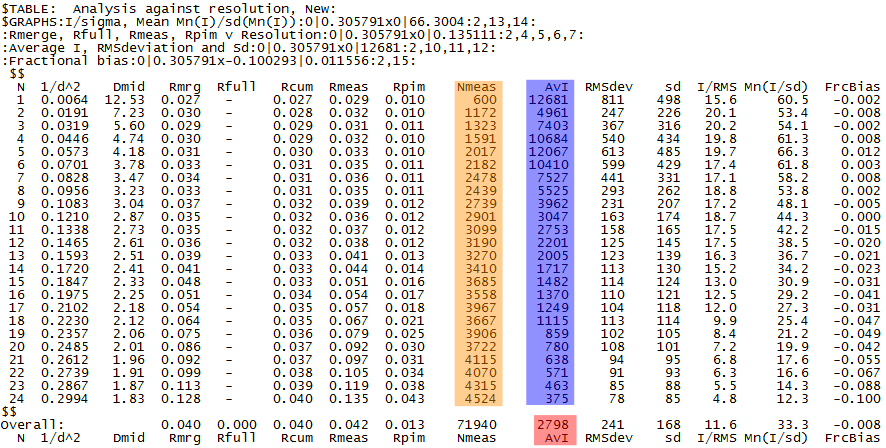
\includegraphics[width=1\textwidth]{figures/dwd/aimlesslog.png}
    \caption[Resolution analysis table from the log file of an AIMLESS job.]{A table given in the log file of an AIMLESS job from an insulin crystal.
    The table gives data for 24 resolution bins including the number of measured reflections in each resolution bin, Nmeas (highlighted orange), and the Average Intensity in each resolution bin, AvI (highlighted blue).
    The value highlighted in red is the overall average intensity for a dataset calculated using reflections that are measurable in that data set.}
    \label{fig: AIMLESS log file}
\end{figure}

\begin{figure}
  \centering
    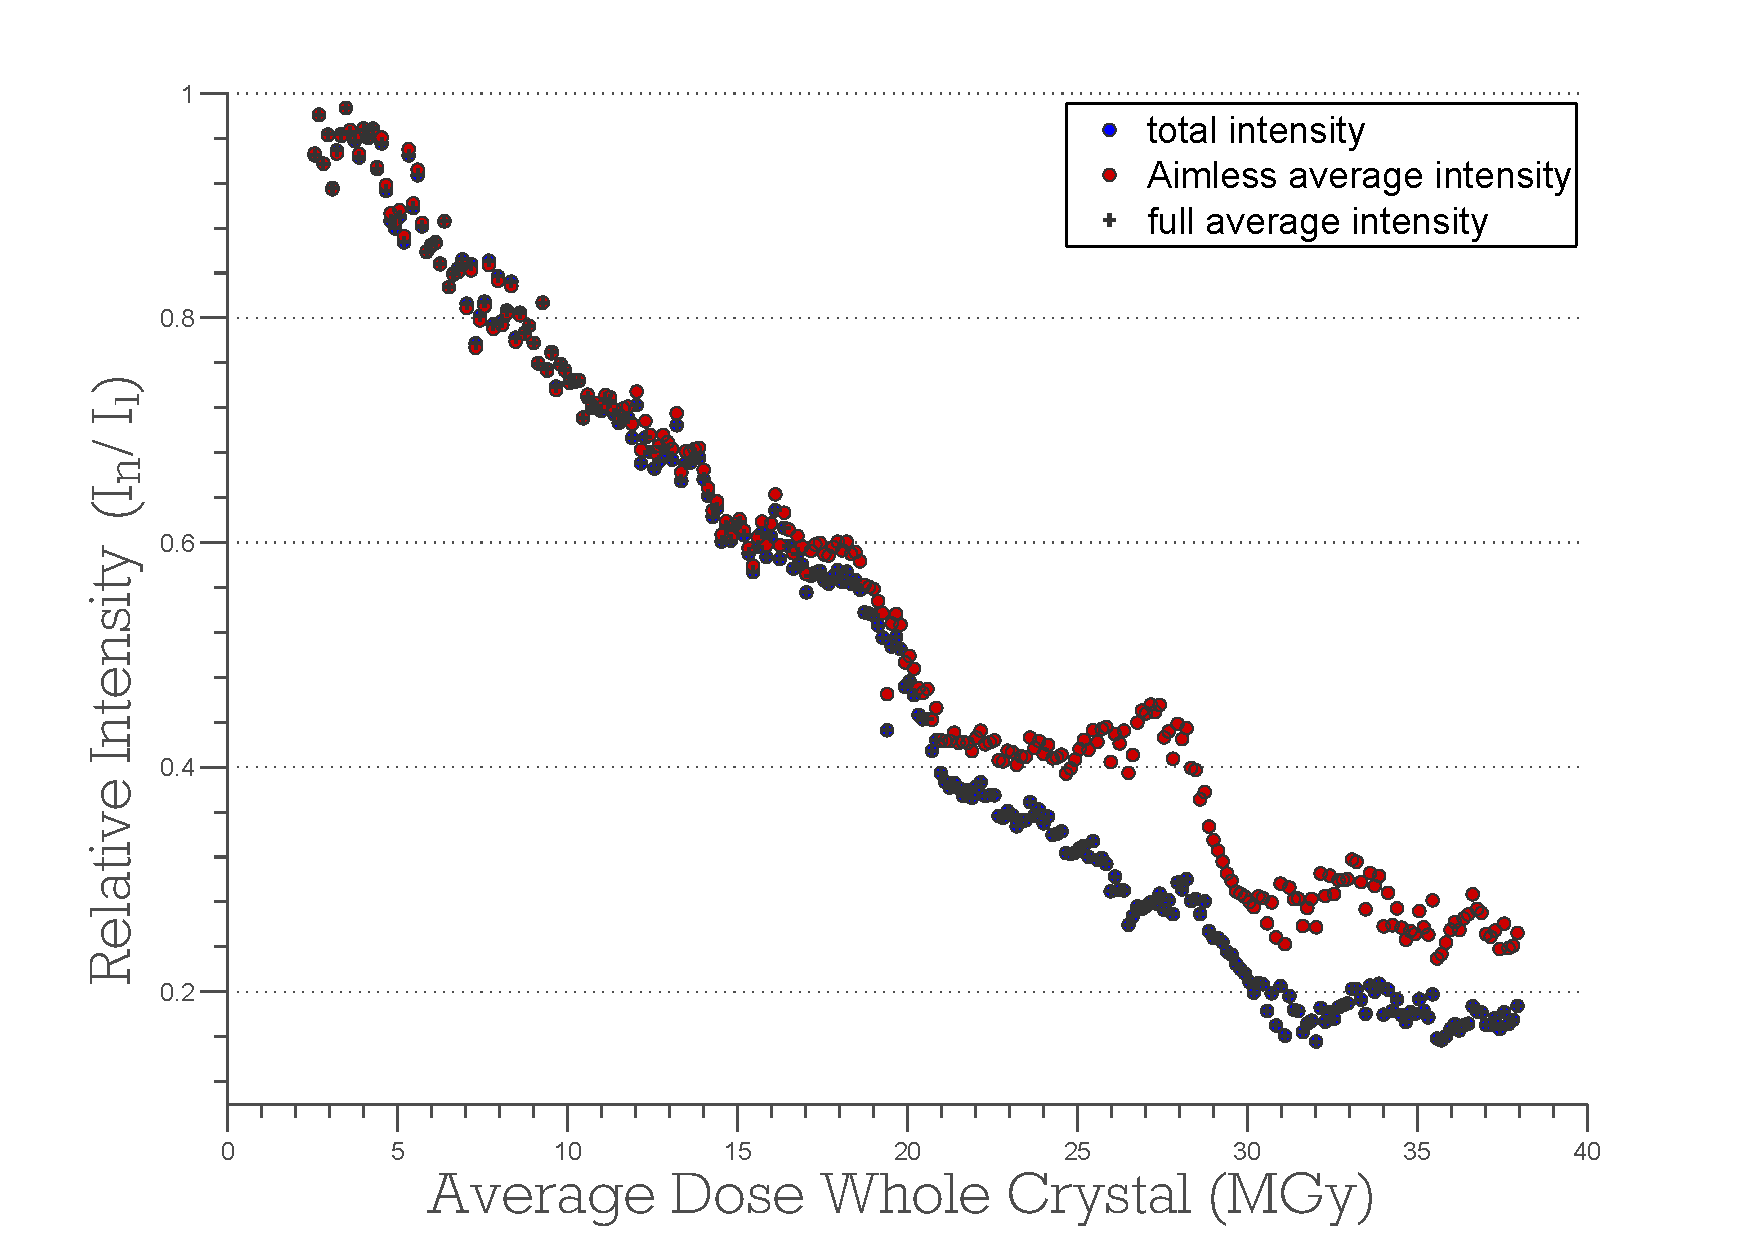
\includegraphics[width=1.0\textwidth]{figures/dwd/calcrelint.pdf}
    \caption[Relative intensity plotted against the average absorbed dose for one insulin crystal.]{Relative intensity plotted against the average absorbed dose for one insulin crystal. The data show that using the overall mean intensity given in the AIMLESS log file increases the relative intensity values because it excludes reflections that cannot be measured. On the other hand, calculating the overall mean intensity using all of the measured reflections from the first data set, agrees with the relative intensity calculated by taking the ratio of the total summed intensity of the current data set divided by that of the first data set.}
    \label{figrelint}
\end{figure}
